\documentclass{IEEEtran}

\usepackage{graphicx}
\usepackage{caption}
\usepackage{subcaption}
\usepackage{hyperref}
\usepackage{url}

\bibliographystyle{plain}

\begin{document}

\title{Computational Psycholinguistics --- Assignment 2}
\author{Daan Brugmans (S1080742)}
\date{\today}

\graphicspath{{./images}}

\maketitle

\section{Introduction}
This report is the realization of the Assignment 2 project for the Radboud University course \href{https://www.ru.nl/courseguides/arts/courses/ma/rema-lc/let-rema-lcex28/}{Computational Psycholinguistics}.
For this assignment, students must investigate whether the gradients computed from a recurrent neural network correlate with measured P600 component activity from a controlled experiment.
The reasoning behind this assignment is that recent research (\cite{fitz2019erp,frank2024gradients}) has shown that the P600 component may be the backpropagation of prediction errors in the human language system.
Since neural language models also backpropagate their prediction errors using gradients, there may exist similarities between the language error backpropagation of human and artificial neural language systems.
This report contains the findings found by me for the Assignment 2 project.

The relevant code for this assignment can be found at the following URL: \url{https://github.com/daanbrugmans/ru-computational-psycholinguistics-23-24/tree/main/assignment-2/code}.

\section{Related Work}
For the Assignment 2 project, students must choose a controlled experiment where participants read English or Dutch sentences while their P600 component is measured.
I have chosen to use the data from the controlled experiment performed in \cite{frank2015erp}.
This data is also used by the authors of \cite{frank2024gradients}, and is briefly introduced in the description of the Assignment 2 project.
This means that my report is (an attempt at) an extension of the work in \cite{frank2024gradients}.

The data from the controlled experiment in \cite{frank2015erp} consists of EEG data of 24 native British English speakers, who all read a set of 205 sentences taken from English-language novels.
The authors recorded EEG data of six different ERP components, including the P600 component, and calculated the average EEG values for every ERP component, for every word of every sentence for every participant of the experiment.
This dataset should fulfill the requirements set by the assignment: the experiment language is English, the participants' stimuli are independent sentences, the size of the P600 component is one dependent variable and showed an effect, and the independent variables are manipulated by varying the content of the sentence stimuli.

\section{Methodology}
All the code I have written can be found in the Jupyter Notebook called \texttt{main.ipynb}, which should thusly contain all results also shown in this report.
It can be found at the following URL: \url{https://github.com/daanbrugmans/ru-computational-psycholinguistics-23-24/blob/main/assignment-2/code/main.ipynb}
I have placed the code in the \texttt{get\_predictions.py} file in a function called \texttt{get\_predictions}, so that I can easily call this code from the notebook.

The dataset of the study in \cite{frank2015erp} is openly accessible through a collection of \texttt{.mat} files, which are typically used in a MatLab setting, but I use Scipy to open this data.
Within the collection of code I hand in alongside this report, the raw data file can be found in the \texttt{data} folder as \texttt{code/data/stimuli\_erp.mat}.
The original README provided by the authors is also included.
From this dataset, I collect the list of sentences read by the participants of the study, and the relevant ERP data.
Although this data does not need any preprocessing, I do wrangle the ERP into the format used by the code in \texttt{get\_predictions.py}, so that I can easily merge the data from the study with the data generated by the models.
I also write the sentence data from the study to a plain text file in the \texttt{items} folder called \texttt{stimuli.txt}, as is required for generating model results.

The data from \cite{frank2015erp} includes the P600 component for all 24 participants per word.
I have chosen to take the mean of all 24 P600s and only analyse these means.
I made this decision because I wanted to have a single P600 for every word to represent the entire participant population.
I have chosen the mean as opposed to the median because of its sensitivity of outliers: I wanted to include information about participants with outlying P600 values for specific words into the aggregated P600 value, and I think that the mean does a better job at this than the median due to its sensitivity to outliers.

My results are a collection of scatterplots that visualize the relationship between 3 variables on the sentence data: the Mean P600 Component, the Surprisal of a Model, and the Gradient Values of a Model.
Every plot also contains a quadratic function fitted to the data to show the trend of the relationship between the variables.
I have chosen for a quadratic function as opposed to a linear function, as I found that this fits the data better.
Included in every plot is also the Pearson Correlation Coefficient \textit{r} between variables.
Since surprisal values and gradients are calculated for multiple models, I provide a plot for every model.
For every pair of variables, I also provide a plot of how the Pearson Correlation Coefficient changes as the model is trained on more data, which will be the main focus of my results.

Before producing results, I set a universal seed for Python itself, NumPy, and PyTorch of \texttt{3131}.
I do this in order to improve the reproducibility of my results.
This is why I also set some settings for CUDA regarding PyTorch's randomness when computing on GPU.

\section{Results}
\begin{figure*}
    \centering
    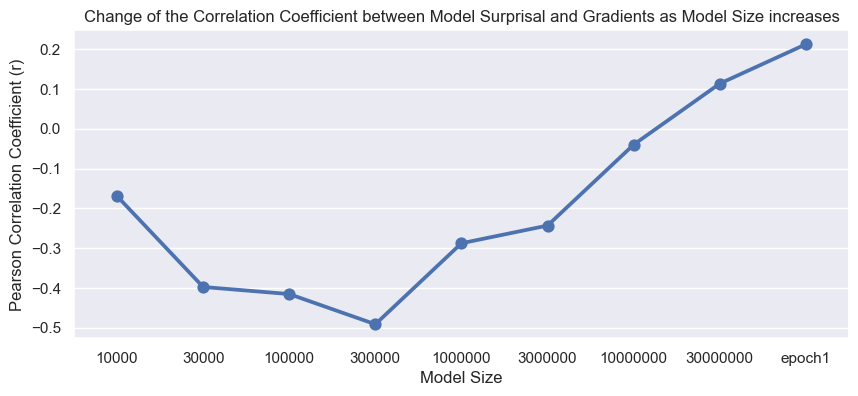
\includegraphics[width=.9\textwidth]{correlation_change/surprisal_gradients.png}
    \caption{The change of the Pearson Correlation Coefficient between Model Surprisal and Model Gradients as the model is trained on increasingly more data.}
    \label{fig:coefficient_surprisal_gradients}
\end{figure*}
\begin{figure*}
    \centering
    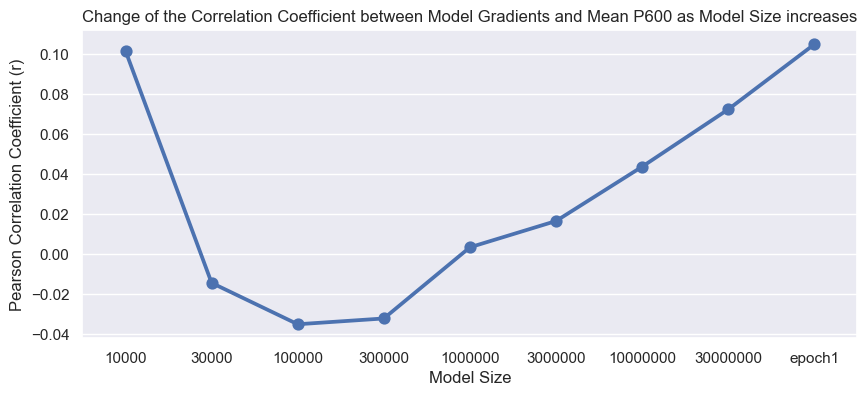
\includegraphics[width=.9\textwidth]{correlation_change/gradients_p600.png}
    \caption{The change of the Pearson Correlation Coefficient between Model Gradients and P600 as the model is trained on increasingly more data.}
    \label{fig:coefficient_gradients_p600}
\end{figure*}
\begin{figure*}
    \centering
    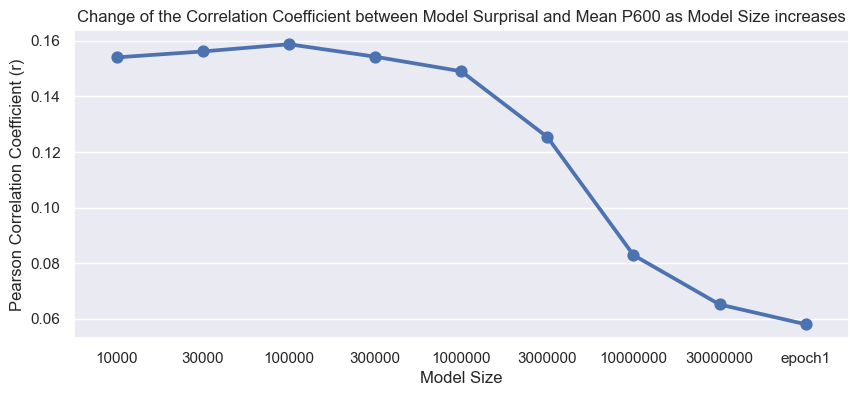
\includegraphics[width=.9\textwidth]{correlation_change/surprisal_p600.png}
    \caption{The change of the Pearson Correlation Coefficient between Model Surprisal and Mean P600 as the model is trained on increasingly more data.}
    \label{fig:coefficient_surprisal_p600}
\end{figure*}

Figures \ref{fig:coefficient_surprisal_gradients}, \ref{fig:coefficient_gradients_p600}, and \ref{fig:coefficient_surprisal_p600} show the change of the correlation between variables as the amount of data the neural language model has trained on increases.
The exact values of the points in this plot can be found in tables \ref{tab:correlation_surprisal_gradients}, \ref{tab:correlation_gradients_p600}, and \ref{fig:coefficient_surprisal_p600} respectively.
The individual scatterplots are placed in the appendices.

The data in figure \ref{fig:coefficient_surprisal_gradients} shows an interesting trend in the predictive power of a model's surprisal 

\begin{table}
    \centering
    \begin{tabular}{c|c}
        \textbf{Trained Data Count} & \textbf{\textit{r}} \\
        \hline
        10000&-0.169\\
        30000&-0.397\\
        100000&-0.415\\
        300000&-0.491\\
        1000000&-0.288\\
        3000000&-0.243\\
        10000000&-0.040\\
        30000000&0.113\\
        epoch1&0.212
    \end{tabular}
    \caption{Correlation Coefficients between Model Surprisal and Model Gradients by the model's train data size.}
    \label{tab:correlation_surprisal_gradients}
\end{table}
\begin{table}
    \centering
    \begin{tabular}{c|c}
        \textbf{Trained Data Count} & \textbf{\textit{r}} \\
        \hline
        1000&0.103\\
        30000&-0.026\\
        100000&-0.035\\
        300000&-0.037\\
        1000000&0.007\\
        3000000&0.021\\
        10000000&0.053\\
        30000000&0.084\\
        epoch1&0.116
    \end{tabular}
    \caption{Correlation Coefficients between Model Gradients and Mean P600 by the model's train data size.}
    \label{tab:correlation_gradients_p600}
\end{table}
\begin{table}
    \centering
    \begin{tabular}{c|c}
        \textbf{Trained Data Count} & \textbf{\textit{r}} \\
        \hline
        10000&0.154\\
        30000&0.156\\
        100000&0.159\\
        300000&0.154\\
        1000000&0.149\\
        3000000&0.125\\
        10000000&0.083\\
        30000000&0.065\\
        epoch1&0.058
    \end{tabular}
    \caption{Correlation Coefficients between Model Surprisal and Mean P600 by the model's train data size.}
    \label{tab:correlation_suprisal_p600}
\end{table}

\section{Conclusions}


\bibliography{bib}

\onecolumn
\appendix
\section{Plots of Model Surprisal vs. Model Gradients}
% \begin{figure}
%     \centering
%     \includegraphics[width=*\textwidth]{}
%     \caption{}
%     \label{fig:}
% \end{figure}

\section{Plots of Model Surprisal vs. Mean P600 Component}

\section{Plots of Model Gradients vs. Mean P600 Component}

\end{document}